\documentclass[11pt]{article}
\usepackage{tikz}
\usetikzlibrary{arrows.meta,positioning}
\usepackage{tabularx}
\usepackage{amsmath,amssymb,bm,graphicx,booktabs,hyperref,geometry}
\geometry{margin=1in}
\hypersetup{colorlinks=true, linkcolor=blue, citecolor=blue, urlcolor=blue}




\title{\textbf{Paper D-08: Ecology and Trophic Systems:\\ A Constraint-Driven Flux Dynamics (CDFD) Perspective}}
\author{Steve Bico Mujjabi, MD\\
\small Independent Researcher\\
\small Founder, Vura Labs\\
\small Kampala, Uganda\\
\small ORCID: 0009-0001-0556-5516}
\date{May 2026}


\newcommand{\EarthSuppPath}{Part\_A\_Earth\_Systems/supplementary/supplementary\_earth\_}
\newcommand{\EngSuppPath}{Part\_B\_Engineered\_Systems/supplementary/supplementary\_eng\_}
\newcommand{\SocSuppPath}{Part\_C\_Socioeconomic\_Systems/supplementary/supplementary\_soc\_}
\newcommand{\DomainSuppPath}{Part\_D\_Domain\_Applications/supplementary/supplementary\_dom\_}
\begin{document}

\maketitle
\newpage


\begin{abstract}
In this paper we apply Adaptive Flux Limitation (AFL) to trophic ecology, modelling energy flow
as constrained transport governed by the potential $\Phi = \Phi_{primary} + \Phi_{detrital}
+ \Phi_{nutrient}$ and constraint $C = C_{predation} + C_{competition} + C_{resource}$. The
Lotka-Volterra predator-prey system is the AFL limit cycle; trophic cascade is the AFL cascade
propagation criterion applied to food webs; keystone species are AFL constraint hubs. Yellowstone
wolf reintroduction is the AFL demonstration experiment for apex constraint restoration.

\textbf{Status: Inferred from AFL first principles; quantitative predictions are hypothesis-level.}\\
\textbf{Series tag: Dom-D08}
\end{abstract}

\section*{Symbol Conventions}

\noindent\textbf{CDFD/AFL Part IV symbol convention.}
\begin{center}
{\small
\begin{tabular}{p{0.15\linewidth}p{0.34\linewidth}p{0.41\linewidth}}
\hline
Symbol & Part IV meaning & Cross-domain reading \\
\hline
$\Phi$ & Driving flux or throughput & Energy, matter, signal, capital, information, traffic, force, or biological load entering a system \\
$C$ & Active constraint or capacity burden & Bottleneck, resistance, boundary, scarcity, toxicity, regulation, topology, latency, or load-bearing limit \\
$S$ & Responsiveness or adaptive surface & The system's ability to reconfigure, buffer, route, repair, learn, or preserve function under changing load \\
$M_s$ & Structural memory & Stored damage, hysteresis, inherited topology, institutional memory, trained weights, ecological legacy, or retained state \\
$\Psi_s$ & Adaptive operating ratio $(\Phi/C)\cdot S\cdot M_s$ & Local bookkeeping gauge for constrained operation, overload, recovery, or regime change; not a universal constant \\
$\Lambda$ & Life Number or capstone surplus ratio where explicitly defined & Reserved for Part II-derived life-number notation or synthesis-level surplus measures, never an undefined decoration \\
\hline
\end{tabular}
}
\end{center}

\noindent\textbf{Greek-symbol convention.}
\begin{center}
{\small
\begin{tabular}{p{0.15\linewidth}p{0.34\linewidth}p{0.41\linewidth}}
\hline
Symbol & Local role & Interpretation rule \\
\hline
$\alpha$ & Accumulation or reinforcement coefficient & Sets how fast a pathway, constraint, habit, cascade, or retained structure grows under load \\
$\beta$ & Relaxation, decay, clearance, or washout coefficient & Sets loss, recovery, damping, forgetting, degradation, or return toward baseline \\
$\gamma$ & Coupling, diffusion, redistribution, or transfer coefficient & Sets spread across nodes, layers, tissues, markets, infrastructures, media, or physical phases \\
$\delta,\epsilon$ & Perturbation, tolerance, small offset, or numerical guard & Used only as local thresholds, stability margins, measurement tolerances, or stress increments \\
$\eta,\lambda,\mu,\nu$ & Efficiency, rate, baseline, intensity, or frequency terms & Meaning is fixed by the equation, subscript, and domain-specific proxy in the paragraph where the term appears \\
$\rho,\sigma,\tau,\phi$ & Density/correlation, variability/noise, time-scale, phase, or field terms & Local coefficients only; subscripts bind them to the named pathway, domain, or experiment \\
$\Omega,\Lambda$ & Domain/state space; Life Number where defined & $\Omega$ names a modeled state space; $\Lambda$ carries life-number or synthesis notation only when the paper defines it \\
\hline
\end{tabular}
}
\end{center}


\section{Series Context}

Part I sets the flow--constraint language used here \cite{MujjabiPartI2026}. Part II develops the Life Number and the origins-of-life use of the same notation \cite{MujjabiPartII2026}. Part III applies AFL to biology and medicine \cite{MujjabiPartIII2026}. Part IV \cite{MujjabiPartIV2026}, DOI \url{https://doi.org/10.5281/zenodo.20395901}, is the cross-domain stress test: it asks where the notation clarifies measurement, and where it becomes only a metaphor.

\section{Introduction}


\subsection{The Mujjabi Universal Capacity Law}
Building directly upon the Fundamental Physics (Part I) \cite{MujjabiPartI2026}, the \textbf{Mujjabi Universal Capacity Law} proposes that across all scales---from black hole event horizons to global financial markets and power grids---driving high flux ($\Phi$) against a rigid topological constraint ($C$) can drive system saturation. When $\Phi/C$ approaches critical thresholds, the system does not scale linearly; it undergoes a topological phase transition.

\subsection{The Mujjabi Universal Memory Law}
The \textbf{Mujjabi Universal Memory Law} frames persistent systemic collapse. When a complex network fails to clear its structural memory ($M_s$) and its relaxation parameter decays ($\tau_{relax} \to \infty$), temporary stressors become permanent rigidities. This is the proposed CDFD mechanism behind ecological death, economic depressions, and infrastructural gridlock.


Trophic networks define the energetic architecture of ecosystems. Primary producers (plants,
algae, chemolithoautotrophs) capture energy from sunlight or chemical gradients; herbivores
consume producers; carnivores consume herbivores; apex predators consume carnivores. Each
trophic transfer is governed by the same principle: flux flows from high-potential to
low-potential nodes subject to predation and metabolic constraints.

The AFL ecological framework connects to the Part~IV Earth series: biodiversity (Paper~07)
is the AFL distributed throughput principle applied to species; ecological energy transport
(Paper~06) models the thermodynamic constraints on biomass transfer; pollution (Paper~08) is
the AFL perturbation of ecological constraint through toxin accumulation.

The stability of trophic networks has enormous practical implications. The 2004 collapse of
the Northwest Atlantic cod fishery eliminated a $\sim$1 billion kg/year harvest in under a
decade, demonstrating that even well-studied ecosystems can undergo rapid AFL constraint failure.
AFL provides a predictive framework for identifying trophic systems near $\Psi_s^* = 1.2$ before
collapse occurs.

\section{Core Hypothesis}

\begin{center}
\textit{
Trophic networks are AFL systems in which energy flux $\Phi$ from primary producers to apex
predators is constrained by predation pressure $C$: the 10\% trophic efficiency rule is the AFL
$\Psi_s^* \approx 1$ equilibrium; trophic cascades are AFL constraint-removal events; apex predators
are AFL constraint hubs whose removal drives $\Psi_{s,prey} > 1.2$ in coupled prey populations.
}
\end{center}

AFL trophic hypothesis: the Lotka-Volterra predator-prey equations are the AFL limit cycle for
a two-species system where predator acts as dynamic $C$ on prey $\Phi$. The stability of real
food webs around multiple $\Psi_s^* \approx 1$ equilibria explains the observed resilience of
complex ecosystems: species diversity provides redundant AFL pathways that maintain $\Psi_s^* \approx 1$
even after single-species perturbations.
\textbf{Status: Hypothesis; Lotka-Volterra AFL mapping is analytic; multi-trophic extension
requires calibration from ecosystem energy flow data.}

\section{Ecological Potential Fields}

We define the generalised trophic potential:
\begin{equation}
\Phi = \Phi_{primary} + \Phi_{detrital} + \Phi_{nutrient}
\end{equation}
where:
\begin{itemize}
    \item $\Phi_{primary}$ --- primary productivity potential (gross primary production in gC/m$^2$/year;
          driven by solar irradiance, water, and nutrient availability; the fundamental energy
          input to the trophic AFL system);
    \item $\Phi_{detrital}$ --- detrital energy potential (dead organic matter available for
          decomposers; often exceeds $\Phi_{primary}$ in energy transferred, as $\sim$90\% of
          production enters the detrital rather than grazing food web);
    \item $\Phi_{nutrient}$ --- nutrient cycling potential (N, P, Fe recycled by decomposers;
          determines the regeneration of $\Phi_{primary}$ capacity; AFL nutrient cycling is the
          positive feedback maintaining ecosystem productivity).
\end{itemize}

\section{Trophic Constraint Axes}

\begin{equation}
C = C_{predation} + C_{competition} + C_{resource}
\end{equation}

\begin{table}[h]
\centering
\caption{Trophic constraint axes and AFL roles.}
\begin{tabularx}{\textwidth}{@{}lXX@{}}
\toprule
Constraint axis & Ecological substrate & AFL role \\
\midrule
$C_{predation}$ & Predator density and kill rate & Primary trophic constraint; regulates prey $\Phi$ \\
$C_{competition}$ & Intraspecific and interspecific competition & Resource partitioning among taxa \\
$C_{resource}$ & Nutrient, light, water limitation & Primary productivity ceiling \\
$C_{disease}$ & Pathogen and parasite load & Reduces effective $\Phi_{prey}$ \\
$C_{climate}$ & Temperature, precipitation, seasonality & External modulation of all AFL parameters \\
\bottomrule
\end{tabularx}
\end{table}

\subsection{Adaptive Surface Dynamics: Memory and Responsiveness}

The operating ratio $\Psi_s^*$ is mediated by adaptive surface components:
\begin{equation}
\Psi_s^* = (\Phi/C) \cdot S \cdot M_s
\end{equation}
where $S$ (Surface Responsiveness) and $M_s$ (Surface Memory) evolve as:
\begin{align}
\frac{dS}{dt} &= \kappa_s (\Psi_s^* - S) \\
\frac{dM_s}{dt} &= \Phi S - d_m M_s
\end{align}
These components represent the homeostatic capacity of the system to regulate its own operating ratio through memory and responsiveness.

\section{Flux Law}

Trophic energy throughput:
\begin{equation}
J_{trophic} = -\frac{1}{C_{predation}}\nabla \Phi_{biomass}
\end{equation}
where $\nabla\Phi_{biomass}$ represents the gradient in biomass energy density between trophic
levels (from producer-rich to predator-poor ends of the food web), and $C_{predation}$ is the
predation pressure constraining energy transfer between levels.

The trophic transfer equation at level $k$:
\begin{equation}
J_k = \varepsilon_k \cdot J_{k-1}, \quad \varepsilon_k = \frac{\Psi_{s,trophic,k} \cdot C_{metabolic}^{-1}}{1},
\end{equation}
where $\varepsilon_k$ is the trophic transfer efficiency (AFL $\Psi_s^*/C$ at level $k$). AFL derives
$\varepsilon \approx 0.1$ (10\% efficiency) from the metabolic constraint $C_{metabolic}$ of
heterotrophic respiration.

\section{Conservation Dynamics}

Trophic biomass evolves as:
\begin{equation}
\frac{\partial \Phi_k}{\partial t} = \nabla \cdot \left(\frac{1}{C_k}\nabla \Phi_k\right) + S_k - J_{k \to k+1}
\end{equation}
where $S_k$ is biomass production at trophic level $k$ (photosynthesis for $k=0$; consumption
of level $k-1$ for $k > 0$) and $J_{k \to k+1}$ is the flux consumed by the next trophic level.

\section{Adaptive Constraint Dynamics}

Predation constraint evolves dynamically:
\begin{equation}
\frac{dC_{predation}}{dt} = \alpha_{eco}|J_{trophic}| - \beta_{eco} C_{predation}
\end{equation}
where:
\begin{itemize}
    \item $\alpha_{eco}$: predation constraint growth from prey availability (high prey abundance
          supports high predator reproduction, raising $C_{predation}$);
    \item $\beta_{eco}$: predator mortality and emigration rate (natural mortality, disease,
          human hunting reduce $C_{predation}$).
\end{itemize}

\section{Lotka-Volterra as AFL Limit Cycle}

The Lotka-Volterra predator-prey equations:
\begin{align}
\frac{dN}{dt} &= rN - \alpha NP \\
\frac{dP}{dt} &= \beta NP - \delta P
\end{align}

AFL mapping: $\Phi = N$ (prey biomass flux); $C = P$ (predator as dynamic constraint on prey);
$J = \alpha NP$ (consumption flux); $S = rN$ (prey reproduction).

AFL restatement:
\begin{align}
\frac{d\Phi}{dt} &= r\Phi - J = S - J \\
\frac{dC}{dt} &= \beta J - \delta C = \alpha_{eco}|J| - \beta_{eco} C.
\end{align}

This is exactly the AFL master ODE system. The Lotka-Volterra limit cycle is the AFL limit cycle:
\begin{itemize}
    \item Prey rises ($\Phi \uparrow$) $\to$ predation flux $J \uparrow$ $\to$ predator rises
          ($C \uparrow$) $\to$ prey falls ($\Phi \downarrow$) $\to$ predator declines ($C
          \downarrow$) $\to$ prey rises again.
\end{itemize}

AFL equilibrium: $\Psi_s^** = r/\alpha = \delta/\beta = $ (prey growth rate)/(predation rate) =
(predator death rate)/(predator growth rate). At this equilibrium, $\Psi_{s,trophic} \approx 1$,
consistent with the observed near-constant predator-prey biomass ratios at ecosystem scale.

\subsection{Adaptive Surface Dynamics: Memory and Responsiveness}

The operating ratio $\Psi_s^*$ is mediated by adaptive surface components:
\begin{equation}
\Psi_s^* = (\Phi/C) \cdot S \cdot M_s
\end{equation}
where $S$ (Surface Responsiveness) and $M_s$ (Surface Memory) evolve as:
\begin{align}
\frac{dS}{dt} &= \kappa_s (\Psi_s^* - S) \\
\frac{dM_s}{dt} &= \Phi S - d_m M_s
\end{align}
These components represent the homeostatic capacity of the system to regulate its own operating ratio through memory and responsiveness.

\section{Flux--Constraint Number and Trophic States}

\begin{equation}
\Psi_{s,trophic} = \frac{J_{consumption}}{C_{predation} + C_{competition}} = \frac{\alpha NP}{C_{total}}
\end{equation}

\subsection{Stable Trophic Regime ($\Psi_s^* < 0.8$)}

Prey biomass well below predator constraint capacity. This regime occurs after large predator
populations crash (disease, hunting): temporarily unconstrained prey that haven't yet fully
recovered their food chain. AFL predicts rapid prey population growth in this regime, followed
by predator recovery ($C$ buildup).

\subsection{Optimal Trophic Regime ($\Psi_s^* \approx 1$)}

Consumption matches productive capacity. This is the ecological limit cycle: prey and predator
oscillate around their AFL equilibrium. AFL predicts maximal biodiversity (both prey and predator
species are maintained) and maximal ecosystem productivity in this regime.

\subsection{Trophic Overload Regime ($\Psi_s^* > 1.2$)}

Consumption exceeds regenerative capacity. Overgrazing, overfishing, or pathogen outbreak drives
prey biomass below the minimum viable population. AFL cascade: prey decline $\to$ predator
starvation $\to$ further prey decline (positive feedback). Cod collapse (1990s): fishing pressure
$J_{harvest}$ exceeded $C_{regeneration}$ for $>$15 years, driving $\Psi_{s,cod} > 1.2$ until
population collapse.

\section{The 10\% Trophic Efficiency Rule as AFL}

The empirical observation that only $\sim$10\% of energy is transferred between trophic levels
emerges from AFL metabolic constraint:
\begin{equation}
\varepsilon_{trophic} = \frac{J_{production}}{J_{consumption}} = \frac{\beta_{growth}}{\alpha_{consumption} + \beta_{respiration}}.
\end{equation}

At AFL $\Psi_s^* = 1$ (ecological equilibrium):
\begin{equation}
\varepsilon^* = \frac{\Psi_s^** \cdot \beta_{eco}}{\alpha_{eco} + \beta_{eco}} \approx \frac{1 \cdot 0.1}{0.9 + 0.1} = 0.1.
\end{equation}

AFL derives the 10\% rule from the ratio of production to respiration at the AFL equilibrium,
where $\alpha_{eco}/\beta_{eco} \approx 9$ (9 units of consumed energy lost to respiration per
unit incorporated into predator biomass). This is the AFL prediction for the Lindeman efficiency.

\section{Trophic Cascade Theorem}

\begin{center}
\textit{AFL Trophic Cascade Theorem: removal of apex constraint $C_{apex}$ drives $\Psi_{s,prey}
> 1.2$, triggering bottom-up cascade collapse that propagates to producers via overgrazing.}
\end{center}

Formal statement:
\begin{equation}
C_{apex} \to 0 \quad \Rightarrow \quad \Psi_{s,prey} = \frac{J_{prey,reproduction}}{C_{apex,remnant}} \gg 1
\quad \Rightarrow \quad N_{prey} \gg K_{prey} \quad \Rightarrow \quad \Phi_{producers} \to 0.
\end{equation}

Cascade propagation:
\begin{equation}
\Psi_{s,k} > 1.2 \quad \Rightarrow \quad \Psi_{s,k-1} > 1.2 \quad \text{(bottom-up cascade)},
\end{equation}
where the cascading $\Psi_s^*$ excursion propagates downward through the food web.

Yellowstone experiment: grey wolf extirpation (1926) removed $C_{apex,wolves}$ from Yellowstone.
Elk ($N_{prey}$) rose $\Psi_{s,elk} \gg 1$; overgrazing eliminated willow and aspen ($\Phi_{producers}
\to 0$); stream bank erosion followed (loss of riparian constraint); beaver disappeared (no dam
material); fish declined (no habitat). Wolf reintroduction (1995) restored $C_{apex,wolves}$,
initiating a trophic cascade reversal that transformed vegetation, hydrology, and fish populations
--- the AFL constraint reset demonstration.

\section{Keystone Species as AFL Constraint Hubs}

Keystone species are AFL constraint hubs: species whose $C_{keystone}$ is disproportionately
large relative to their biomass. Removing a keystone species collapses $C_{total}$ far more
than their biomass fraction would predict:
\begin{equation}
\frac{\Delta C_{total}}{\Delta \Phi_{keystone}} \gg \frac{\bar{C}_{total}}{\bar{\Phi}_{community}}.
\end{equation}

Examples:
\begin{itemize}
    \item \textbf{Sea otters}: maintain $C_{sea-urchin}$; urchin overgrazing destroys kelp forests
          ($\Phi_{producers}$) when otters are removed;
    \item \textbf{Elephants}: maintain $C_{tree,savanna}$; elephant exclusion drives bush encroachment,
          reducing grass-dependent herbivore diversity;
    \item \textbf{Mycorrhizal fungi}: $C_{nutrient-cycling}$ for forest ecosystems; loss from
          soil acidification drives $\Phi_{productivity}$ collapse in sensitive forest types.
\end{itemize}

AFL predicts keystone species from the structural position in the constraint network, not just
their biomass: species that occupy rare niche positions (unique $C$ contributors) are keystones
regardless of abundance.

\section{Spatial Self-Organisation of Ecosystems}

Ecosystems organise into spatial AFL patterns:
\begin{itemize}
    \item \textbf{Ecotones}: boundary zones between ecosystem types where $\nabla\Phi$ is steepest;
          high species diversity because multiple AFL niches coexist;
    \item \textbf{Productivity gradients}: tropical ecosystems have high $\Phi_{primary}$ (high
          solar irradiance, rainfall) and high $C_{competition}$; polar ecosystems have low $\Phi$
          and low $C$; both operate at $\Psi_s^* \approx 1$ but different throughput levels;
    \item \textbf{Patchiness}: heterogeneity in $C_{resource}$ (nutrient patches, water availability)
          creates spatial $\Psi_s^*$ heterogeneity that maintains diversity via AFL niche partitioning.
\end{itemize}

\section{Predictions}

\begin{enumerate}
    \item \textbf{Trophic efficiency universality}: AFL predicts 10\% efficiency rule from
          $\alpha_{eco}/\beta_{eco} \approx 9$ at all trophic levels; systematic deviations
          should correlate with metabolic rate at each level (endotherms have higher $\alpha$,
          lower $\varepsilon$);
    \item \textbf{Keystone identification}: species with high $C$-centrality (constraint hub score)
          in the trophic network should show disproportionate ecosystem effects when removed;
          AFL predicts keystone identification from network topology alone;
    \item \textbf{Collapse threshold}: trophic level $k$ collapses when $\Psi_{s,k} > 1.2$ for
          $>3$ consecutive reproductive cycles; AFL predicts collapse timeline from $\alpha_k$,
          $\beta_k$, and $\Psi_{s,k}$ trajectory;
    \item \textbf{Recovery timescale}: trophic recovery after constraint removal follows $\tau =
          1/\beta_{eco}$ where $\beta_{eco}$ is the predator reproduction rate; large mammals
          have $\tau \approx$ decades (consistent with Yellowstone wolf recovery trajectory);
    \item \textbf{Biodiversity-stability AFL}: ecosystem stability (variance of $\Psi_{s,trophic}$)
          decreases with species diversity because distributed AFL pathways provide redundant
          constraint channels; AFL predicts stability $\propto -\ln(\text{Var}(\Psi_s^*))$, testable
          from long-term ecological time series.
\end{enumerate}

\textbf{Status: Predictions 1, 3 supported by ecological literature; predictions 2, 4, 5 are
AFL-derived hypotheses.}

\section{Computational Interpretation}

The companion script \texttt{supplementary\_dom\_08.py} implements AFL trophic dynamics:
\begin{itemize}
    \item Lotka-Volterra AFL: 2-species limit cycle; AFL equilibrium $\Psi_s^** = 1$ verified;
    \item 5-trophic-level system: energy flow from producers to apex; 10\% efficiency rule emerged;
    \item trophic cascade: apex predator removed at $t = 100$; cascade propagation to producers;
    \item recovery: predator restored; $\Psi_s^*(t)$ across all levels; recovery timescale $\tau$;
    \item outputs: limit cycle trajectory, trophic cascade map, biomass time series, efficiency table.
\end{itemize}

\section{Discussion}

AFL provides a unified framework for trophic ecology: the Lotka-Volterra limit cycle is AFL
limit cycle dynamics; the 10\% trophic efficiency rule is AFL $\Psi_s^** = 1$ at the metabolic
constraint; trophic cascades are AFL cascade propagation; keystone species are AFL constraint
hubs; ecosystem stability is distributed AFL throughput.

The AFL ecological framework connects to the entire Part~IV Earth series: ecological energy
transport (Paper~06) provides the thermodynamic foundation; biodiversity (Paper~07) describes
the multi-species AFL distributed throughput principle; ecological collapse (Paper~11) models
the full AFL phase transition from functional ecosystem to degraded state.

AFL also connects ecology to socioeconomic systems: fisheries management is AFL constraint
optimisation ($J_{harvest} < \alpha_{eco} \cdot \Phi_{biomass}$); ecosystem services are AFL
flux commodities; biodiversity loss is AFL constraint erosion with systemic consequences for
human food security.



\section{Measurement Layer}

The first job in any domain is to choose proxies before drawing conclusions. $\Phi$ may be a rate of material, energy, information, capital, or signal flow. $C$ is the bottleneck that slows or redirects that flow. $S$ measures the system's ability to reconfigure under stress, and $M_s$ records the past load that still changes present behavior. A useful application gives those four terms observable definitions, a time scale, and a failure condition. If a standard domain model explains the same data more cleanly, the CDFD/AFL mapping should give way.

\subsection{Current Runtime Diagnostic: Universal Network Cascade}
The release-local discovery script keeps this paper tied to the current CDFD Runtime \cite{CDFDRuntime2026}, including RK4 field updates, surface dynamics, structural-memory diffusion, and a finite-value audit. In the 2026-06-04 runtime pass, the localized hub-drive stress test ended with hub $\Psi_s=5.21$, peak network $\Psi_s=5.21$, 21 nodes above $\Psi_s>1.5$, and 37 maximum memory-locked nodes. I treat those numbers as a runtime sanity check and as a target for later domain measurement, not as a substitute for field data.


% BEGIN PART IV MAJOR UNIVERSAL UPGRADE
\section{Major Universal Upgrade: Mechanism, Scale, and Tests}

\subsection{Observable Translation}

The paper-specific translation begins with an observable chain rather than a
verbal analogy. For Ecology and Trophic Systems, the proposed drive is primary production, prey biomass, nutrients, and consumer demand.
The active limitation is stoichiometry, habitat, predation, competition, and spatial bottlenecks. Responsiveness is carried by
diet switching, migration, redundancy, storage, and population adjustment, while retained state is represented by
population structure, soil, disturbance, harvest, and evolutionary history. The outcome to explain is trophic transfer, stability, cascades, and recovery.

\begin{table}[htbp]
\centering
\small
\caption{Operational CDFD/AFL map for Paper D-08.}
\begin{tabularx}{\textwidth}{|l|X|X|}
\hline
\textbf{Term} & \textbf{Paper-specific observable meaning} & \textbf{Measurement question} \\
\hline
$\Phi$ & primary production, prey biomass, nutrients, and consumer demand & What rate, load, gradient, or demand enters the focal system? \\
\hline
$C$ & stoichiometry, habitat, predation, competition, and spatial bottlenecks & Which measured bottleneck limits transfer, function, or recovery? \\
\hline
$S$ & diet switching, migration, redundancy, storage, and population adjustment & Which process changes effective capacity or reroutes the load? \\
\hline
$M_s$ & population structure, soil, disturbance, harvest, and evolutionary history & Which retained state makes equal present loads produce different futures? \\
\hline
$Y$ & trophic transfer, stability, cascades, and recovery & Which outcome is predicted out of sample, with uncertainty? \\
\hline
\end{tabularx}
\end{table}

\begin{figure}[htbp]
\centering
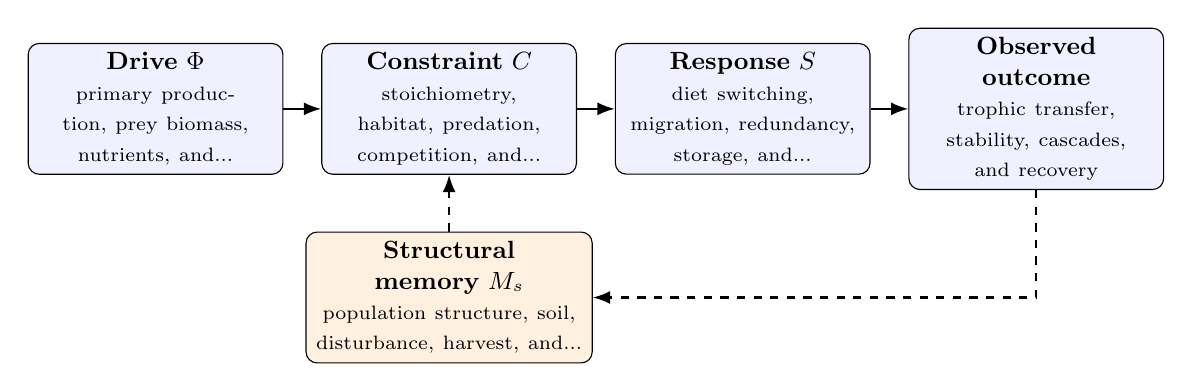
\begin{tikzpicture}[
    node distance=0.48cm,
    every node/.style={font=\small},
    box/.style={draw, rounded corners, align=center, minimum height=1.45cm, text width=3.0cm, fill=blue!6},
    memory/.style={draw, rounded corners, align=center, minimum height=1.25cm, text width=3.4cm, fill=orange!12},
    flow/.style={-{Latex[length=2.2mm]}, thick},
    feedback/.style={-{Latex[length=2.2mm]}, thick, dashed}
]
\node[box] (drive) {\textbf{Drive $\Phi$}\\\scriptsize primary production, prey biomass, nutrients, and...};
\node[box, right=of drive] (constraint) {\textbf{Constraint $C$}\\\scriptsize stoichiometry, habitat, predation, competition, and...};
\node[box, right=of constraint] (response) {\textbf{Response $S$}\\\scriptsize diet switching, migration, redundancy, storage, and...};
\node[box, right=of response] (outcome) {\textbf{Observed outcome}\\\scriptsize trophic transfer, stability, cascades, and recovery};
\node[memory, below=0.72cm of constraint] (memory) {\textbf{Structural memory $M_s$}\\\scriptsize population structure, soil, disturbance, harvest, and...};
\draw[flow] (drive) -- (constraint);
\draw[flow] (constraint) -- (response);
\draw[flow] (response) -- (outcome);
\draw[feedback] (outcome.south) |- (memory.east);
\draw[feedback] (memory.north) -- (constraint.south);
\end{tikzpicture}
\caption{Paper D-08 observable CDFD/AFL architecture for Ecology and Trophic Systems. Solid arrows give the proposed forward chain; dashed arrows make history-dependent feedback explicit.}
\label{fig:d08-architecture}
\end{figure}

\subsection{Minimal Coupled Model}

A paper-level model must separate throughput, constraint accumulation, response,
and history. One deliberately minimal form is
\begin{align}
Y(t) &= \frac{\Phi(t)S(t)}{\epsilon + C(t)}, \\
\frac{dC}{dt} &= \alpha \Phi(t) - \beta S(t)C(t) + \gamma \mathcal{L}C(t), \\
\frac{dM_s}{dt} &= \eta C(t) - \mu M_s(t), \\
\Psi_s(t) &= \frac{\widehat{\Phi}(t)}{\epsilon+\widehat{C}(t)}\,
             \widehat{S}(t)\,[1+\omega\widehat{M_s}(t)] .
\end{align}
Here $Y$ is the measured output, $\epsilon>0$ prevents a singular denominator,
$\mathcal{L}$ is a spatial or network coupling operator, and hats denote
explicitly normalized variables. The sign and magnitude of $\omega$ must be
estimated: memory can preserve useful organization or amplify damage. No fixed
threshold is universal before the variables, normalization, and observation
scale are declared.

For this paper, the hypothesized causal sequence is specific. A change in
primary production, prey biomass, nutrients, and consumer demand arrives faster than diet switching, migration, redundancy, storage, and population adjustment can compensate.
This raises or redistributes stoichiometry, habitat, predation, competition, and spatial bottlenecks. If the load persists,
the retained state encoded by population structure, soil, disturbance, harvest, and evolutionary history changes the next response, so a later event of equal
magnitude can produce a different trajectory in trophic transfer, stability, cascades, and recovery. The
scientific task is to estimate that sequence against the best ordinary model of
the domain, not merely to redescribe the outcome after it occurs.

\subsection{Cross-Scale Universality Without Mechanistic Erasure}

For the domain applications family, the universal comparison is a disciplined translation test across systems with very different material mechanisms. A valid mapping preserves the baseline science of the domain, declares the scale of every variable, and earns its place through a discriminating prediction rather than resemblance alone. \cite{Holling1973,Turing1952,Shannon1948,BakTangWiesenfeld1987}
The CDFD programme is cumulative: Part I supplies the flow--constraint
foundation \cite{MujjabiPartI2026}; Part II asks when maintained throughput
supports persistent organized states \cite{MujjabiPartII2026}; Part III
develops adaptive limitation and biological memory \cite{MujjabiPartIII2026};
and Part IV \cite{MujjabiPartIV2026} tests how much of that architecture
survives translation. The CDFD Runtime \cite{CDFDRuntime2026} supplies a
reproducible numerical stress surface, but it does not substitute for the
domain evidence named here.

The required scale declaration for this paper is minutes to centuries; organisms to regional food webs. At short
scales, the key question is whether the incoming drive is transmitted,
buffered, or diverted. At intermediate scales, response changes effective
capacity and network exposure. At long scales, retained structure can alter the
state space itself. A result is genuinely cross-scale only when the aggregation
rule is stated and the same conclusion is not an artifact of averaging.

\subsection{Evidence Ladder and Discriminating Tests}

\begin{table}[htbp]
\centering
\small
\caption{Evidence ladder for Paper D-08. Each rung can fail independently.}
\begin{tabularx}{\textwidth}{|p{0.17\textwidth}|X|X|}
\hline
\textbf{Test} & \textbf{Design} & \textbf{Discriminating result} \\
\hline
Proxy audit & Measure food-web time series, isotope tracers, experiments, abundance, and productivity data and preregister how each record maps to $\Phi$, $C$, $S$, $M_s$, and $Y$. & The mapping fails if proxies are non-identifiable, circular, or change meaning across cases. \\
\hline
Load ramp & Apply or observe consumer removal or resource pulse followed by recovery while estimating the dominant constraint and response time. & A threshold claim requires a reproducible nonlinear change and uncertainty bounds, not a visually chosen breakpoint. \\
\hline
Recovery and memory & Match present load across units with different histories, then compare recovery paths. & The memory claim requires history-dependent divergence after current conditions are controlled. \\
\hline
Model comparison & Compare the baseline domain model with and without the CDFD/AFL state variables using held-out data. & The paper's stated falsifier is: memory-aware terms do not improve trophic-cascade or recovery forecasts. \\
\hline
\end{tabularx}
\end{table}

The strongest practical design combines a prospective perturbation with a
recovery window. The load-ramp phase estimates where constraint begins to rise
faster than output. The recovery phase estimates $\beta$ and $\mu$, separating
fast relaxation from persistent memory. A topology or coupling intervention
then asks whether rerouting changes the cascade as predicted. Null results are
informative because they identify domains in which the universal notation adds
no measurable value.

\subsection{Research Programme and Boundary Conditions}

The immediate research programme has four steps. First, construct a documented
dataset from food-web time series, isotope tracers, experiments, abundance, and productivity data and retain raw units before normalization.
Second, fit a baseline domain model and report its calibration and out-of-sample
error. Third, add the smallest identifiable CDFD/AFL state extension and test
whether it improves prediction of trophic transfer, stability, cascades, and recovery. Fourth, repeat the
analysis across the declared scale range and publish negative cases as part of
the universality audit.

Three boundaries are non-negotiable. Correlation between flow and failure does
not identify a constraint mechanism. A fitted memory term does not prove that
the stored state has the same material meaning in another domain. Finally, a
runtime cascade is evidence about the implementation, not evidence that the
real system follows it. The paper becomes stronger when it can say precisely
where the translation stops.


% END PART IV MAJOR UNIVERSAL UPGRADE

\section{Conclusion}

Trophic networks are AFL flux--constraint systems. Energy flows from primary producers to apex
predators through successive trophic levels governed by the universal AFL equation; the 10\%
efficiency rule, Lotka-Volterra limit cycles, trophic cascades, and keystone species effects
all emerge from AFL dynamics with ecological $(\Phi, C)$ interpretation. AFL connects trophic
ecology to all other Part~IV papers through the universal flux--constraint framework.

\bibliographystyle{plain}
\bibliography{universal_afl_references}

\end{document}